\documentclass[laporan.tex]{subfiles}

\begin{document}

\chapter{Tinjauan Pustaka}

\section{Penelitian Terkait}

\subsection{Improving quality inspection of food products by computer vision – a review}

Kualitas produk pangan diukur dari penampilan, bau, tekstur, rasa dan berbagai aspek subjektif lainnya yang dinilai oleh manusia. Namun inspeksi dengan tenaga manusia mempunyai banyak kelemahan antara lain ongkos yang tinggi serta  hasil yang tidak konsisten.

Makalah ini\cite{brosnan} membahas berbagai penelitian di bidang computer vision yang diterapkan untuk menggantikan inspeksi manual pada berbagai produk pangan dan pertanian.

Beberapa penelitian memfokuskan pada deteksi cacat bentuk atau tekstur secara visual. Ekspansi Fourier dapat mendeteksi bentuk kultivar apel dengan kesuksesan 90\%.

\subsection{Identifikasi Kematangan Buah Tomat Menggunakan Metoda \emph{Backpropagation}}

Penelitian ini mengidentifikasi kematangan buah tomat melalui pemrosesan data histogram citra dengan jaringan syaraf tiruan (JST). Metode JST yang digunakan adalah \emph{backpropagation} dengan 3 unit input untuk komponen warna RGB, 4 \emph{hidden layer} dan 3 unit output. Dari input nilai histogram ternormalisasi dihasilkan 3 target output yaitu buah masak (1 1 1), setengah masak (0 1 0) dan buah muda (0 0 0).\cite{derisma}

JST \emph{backpropagation} mengenali pola melalui pelatihan dengan data \emph{training} dengan tiga \emph{sample} untuk masing-masing target output (3 \emph{sample} buah matang, 3 \emph{sample} buah mentah dan 3 \emph{sample} buah setengah matang). Pelatihan dilakukan sebanyak 50000 kali untuk mendapatkan nilai bobot yang akan digunakan untuk mengidentifikasi tingkat kematangan buah tomat.

Uji identifikasi dilakukan terhadap 20 data dari masing-masing tipe target. Sistem berhasil mengidentifikasi 85\% buah matang, 45\% buah mentah dan 85\% buah setengah matang. Pengaruh pencahayaan menyebabkan identifikasi buah matang lebih akurat daripada buah mentah.

\subsection{Navel Orange Blemish Identification for Quality Grading System}

Menurut penelitian ini, klasifikasi pixel untuk mengenali memar pada kulit jeruk mempunyai akurasi rendah karena perbedaan intensitas warna antara bagian tengah jeruk dengan bagian tepi jeruk pada citra jeruk. Untuk mengatasi masalah tersebut pengetahuan a priori mengenai variasi intensitas pada benda bulat diterapkan agar pixel bagian yang cacat dapat dikenali dengan tepat.\cite{liu}

Sistem deteksi cacat berusaha meniru persepsi manusia yang membandingkan warna secara relatif dengan warna sekeliling.

Langkah pertama deteksi adalah dengan menggolongkan jeruk berdasarkan kematangan. Algoritma yang digunakan berbeda untuk jeruk matang dan mentah karena adanya variasi warna pada jeruk mentah. Klasifikasi ini dilakukan dengan selisih nilai \emph{threshold} Otsu pada komponen warna merah dan hijau. Jeruk matang mempunyai nilai selisih yang lebih tinggi.

Klasifikasi awal dilakukan pada warna-warna kulit jeruk berdasarkan nilai komponen R, G dan B pada tiap pixel. Nilai yang kurang dari ambang batas berdasarkan algoritma Otsu dianggap tidak ada pada pixel. Berdasarkan kombinasi warna primer, tiap pixel digolongkan menjadi satu dari delapan jenis warna.

\begin{table}[h]
\centering
\begin{tabular}{|c|c|c|c|c|}
\hline
No. & Kelas Warna & R & G & B \\
\hline
1. & Latar belakang & 0 & 0 & 0 \\
2. & Biru & 0 & 0 & 1 \\
3. & Hijau & 0 & 1 & 0 \\
4. & Cyan & 0 & 1 & 1 \\
5. & Merah & 1 & 0 & 0 \\
6. & Magenta & 1 & 0 & 1 \\
7. & Kuning & 1 & 1 & 0 \\
8. & Putih & 1 & 1 & 1 \\
\hline
\end{tabular}
\caption{Tabel Kelas Warna Citra Jeruk}
\label{table:colorclass}
\end{table}

Kelas-kelas tersebut diberi bobot sedemikian rupa sehingga terurut dari intensitas terendah sampai intensitas tertinggi. Hasil eksperimen menunjukkan bahwa kelas warna merah dan magenta tidak ditemukan pada jeruk matang maupun mentah.

Selanjutnya untuk tiap kelas dihitung intensitas rata-rata pada masing-masing komponen warna primer. Jarak antarkelas dihitung dengan \emph{squared mean difference} dari rata-rata intensitas untuk masing-masing komponen, kemudian dirata-rata dengan \emph{quadratic mean}. Dari jarak antarkelas dapat ditemukan adanya beberapa kelas yang bertetangga, yaitu dua kelas yang terdekat satu sama lain. Kelas yang bertetangga digabungkan menjadi kelas baru, sedangkan kelas yang tidak ada pada data dihapus. Dilakukan perhitungan rata-rata intensitas pada kelas baru.

Klasifikasi selanjutnya dilakukan dengan pencarian jarak minimum dari tiap pixel dengan rata-rata intensitas masing-masing kelas baru. Pixel yang masuk pada kelas dengan intensitas tertinggi (\emph{top layer}) dianggap sebagai bagian kulit jeruk yang normal, sedangkan bagian cacat ditentukan dari lubang pada daerah dengan intensitas tertinggi tersebut.

Metode di atas dapat menentukan daerah cacat sebanyak 70\%-80\% pada bagian tengah dari seluruh permukaan jeruk yang tampak pada citra. Deteksi tidak dapat dilakukan pada bagian tepi karena adanya perbedaan intensitas cahaya yang diterima oleh objek.

\section{Computer Vision}

Citra digital adalah fungsi intensitas warna dua dimensi $f(x,y)$, dengan $x$ dan $y$ mewakili koordinat lokasi suatu titik dan nilai dari fungsi yang merupakan tingkat intensitas warna atau tingkat keabu-abuan dari titik tersebut (Schalkoff, 1989). Citra digital merupakan representasi dari suatu objek nyata yang dapat dikenali oleh komputer.

Pengolahan citra digital atau digital image processing pengolahan sinyal untuk input citra digital dua dimensi. Tujuan pengolahan citra digital adalah untuk meningkatkan kualitas gambar sehingga lebih mudah dilihat oleh manusia atau lebih mudah diolah oleh komputer.

Computer vision adalah bidang studi yang mempelajari metode-metode pengumpulan, pemrosesan, analisis dan penafsiran citra dari dunia nyata dengan tujuan untuk menghasilkan informasi numerik atau simbolis.

Berikut ini adalah pengertian computer vision menurut beberapa pakar

\begin{enumerate}
\item Ballard dan Brown, computer vision adalah otomatis dan integrasi sebuah range yang luas yang terdiri dari proses-proses dan representasi-representasi terhadap persepsi visual.
\item Adrian Low, computer vision berhubungan dengan perolehan gambar, pemrosesan, klasifikasi, pengenalan, dan menjadi penggabungan, pengurutan, pembuatan keputusan menuju pengenalan.
\item Shapiro dan Stockman, computer vision adalah suatu bidang yang bertujuan untuk membuat suatu keputusan yang berguna mengenai objek fisik nyata dan keadaan berdasarkan atas sebuah citra. Computer vision merupakan kombinasi antara pengolahan citra dan pengenalan pola. Hasil keluaran dari proses computer vision adalah pengertian tentang citra.
\end{enumerate}

Boyle dan Thomas mengatakan bahwa computer vision lebih daripada pengenalan, computer vision melakukan operasi “low level processing” sebagai algoritma image processing yang murni. Mereka juga yang menggolongkan image processing ke dalam computer vision.

\section{Standard Kualitas Jeruk Menurut SNI 3165-2009}

SNI telah menetapkan standard kualitas untuk buah jeruk keprok (Citrus sinensis) dalam SNI 3165-2009[3]. Standard ini diberlakukan bagi buah jeruk keprok yang dipasarkan untuk konsumsi langsung (bukan olahan atau bahan baku industri). Standard ini meliputi standard minimum, ketentuan kematangan, pengemasan, pelabelan, higienis, cemaran logam berat dan residu pestisida. Setelah memenuhi standard minimum tersebut, jeruk dapat diklasifikasi mutu dan ukurannya dengan batas-batas toleransi untuk tiap kelas mutu.\cite{sni}

Berdasarkan standard SNI tersebut, buah jeruk keprok dibagi menjadi tiga kelas:

\begin{description}
\item [Kelas super] Jeruk keprok bermutu paling baik (super) mencerminkan ciri varietas/tipe komersial, bebas dari kerusakan kecuali kerusakan sangat kecil
\item [Kelas A] Jeruk keprok bermutu baik yaitu mencerminkan ciri varietas/tipe komersial, dengan kerusakan kecil. Total area yang mengalami penyimpangan dan cacat maksimum 10\% total luas permukaan buah dan penyimpangan tersebut tidak boleh mempengaruhi mutu daging buah.
\item [Kelas B] Sama seperti Kelas A dengan toleransi cacat maksimum 15\% dari total luas permukaan buah.
\end{description}

\section{Teori Pendukung}

Metode yang digunakan untuk mendeteksi cacat adalah klasifikasi \emph{pixel} berdasarkan jarak, dengan metode Otsu untuk klasifikasi awal \emph{pixel} yang akan digunakan dalam penentuan titik awal pusat \emph{cluster}. Metode ini dipilih karena tidak membutuhkan \emph{training set} sehingga dapat diterapkan untuk data dalam jumlah terbatas.

\subsection{\emph{Nearest Neighbor Search}}

\emph{Nearest Neighbor Search} (NNS) adalah optimisasi untuk menemukan titik data yang paling mirip. Ukuran kesamaan antara titik-titik data dengan $n$-atribut dapat dideskripsikan dalam fungsi ketidaksamaan \emph{(dissimilarity function)}.\cite{knuth} Pada umumnya data dimodelkan sebagai titik-titik pada ruang vektor dimensi-$n$. Salah satu perhitungan yang digunakan untuk mengukur ketidaksamaan antardata adalah rumus jarak Euclid.

\begin{equation}
	d=\sqrt{\sum_{i=1}^n (a_i - b_i)^2}
\end{equation}

$a_i$ dan $b_i$ adalah atribut ke-$i$ dari $a$ dan $b$.

Untuk keperluan klasifikasi, tiap kelas data diwakili oleh sebuah titik pusat \emph{(centroid)} yang berada di tengah sebuah kelas, dan data yang diuji diklasifikasikan ke kelas yang memiliki titik pusat terdekat dengan data tersebut. Gambar \ref{fig:distex} menunjukkan contoh klasifikasi berdasarkan jarak.

\begin{figure}[h]
\centering
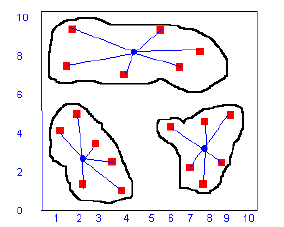
\includegraphics{tex/distex.png}
\caption{Ilustrasi Klasifikasi Berdasarkan Jarak Terdekat}
\label{fig:distex}
\end{figure}

Perhitungan jarak Euclidean digunakan untuk mengklasifikasikan \emph{pixel} pada citra jeruk untuk deteksi daerah cacat. Tiap \emph{pixel} diukur jaraknya dari nilai intensitas rata-rata tiap kelas.

\subsection{Sistem Warna RGB}
Sistem warna atau model warna adalah spesifikasi sistem koordinat dan subruang dalam koordinat tersebut dengan tiap warna direpresentasikan sebagai sebuah titik. Sistem warna RGB memodelkan semua warna sebagai kombinasi tiga warna primer yaitu merah (R), hijau (G) dan biru (B) dalam berbagai intensitas. Dalam model ini, sebuah koordinat kartesius 3-dimensi menunjukkan besarnya intensitas tiap komponen warna. Warna-warna digambarkan sebagai titik-titik di dalam sebuah kubus yang meliputi seluruh kombinasi nilai ketiga komponen, setiap warna dideskripsikan dengan vektor dari titik asal. Warna hitam terletak di titik asal koordinat, dan warna putih di sudut terjauh dari titik asal.

\begin{figure}[h]
\centering
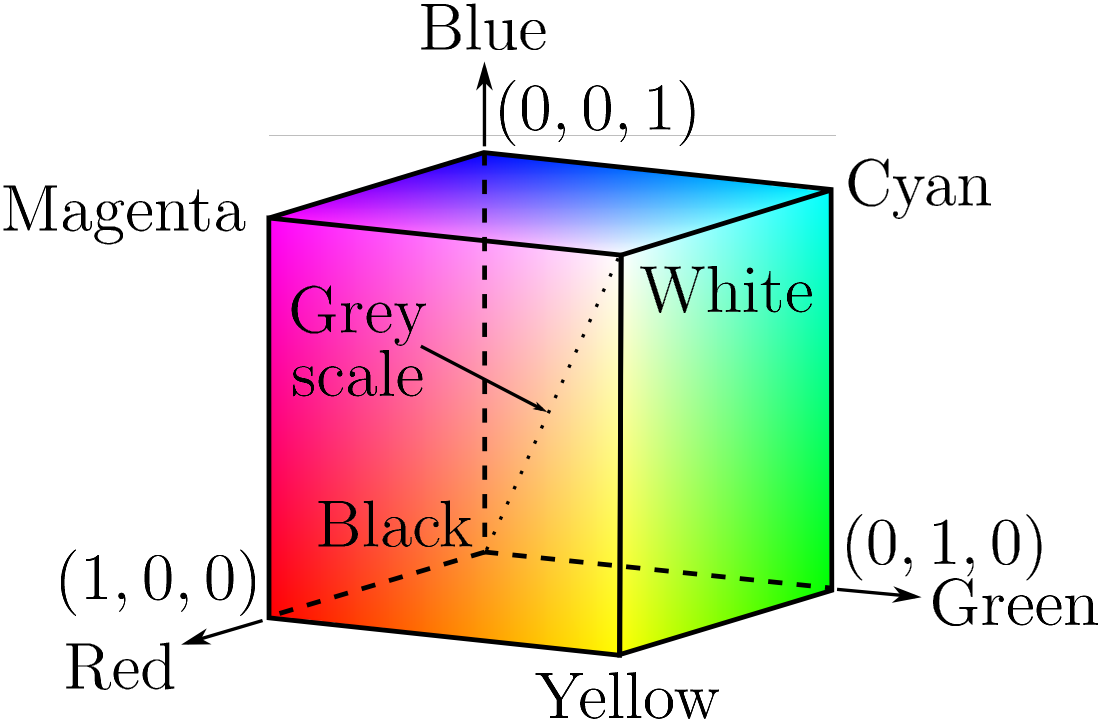
\includegraphics[width=10cm]{tex/rgb-colourcube.png}
\caption{Kubus Model Warna RGB}
\end{figure}

\emph{Pixel} pada citra digital merupakan kombinasi tiga nilai intensitas komponen warna primer RGB, maka tiap \emph{pixel} dapat dilihat sebagi titik-titik data pada koordinat kartesius 3-dimensi dari sistem warna RGB. Sebagaimana titik pada ruang vektor lainnya, ukuran metrik fungsi ketidaksamaan berlaku untuk data \emph{pixel} RGB, sehingga klasifikasi \emph{nearest neighbor} dapat diterapkan.


\subsection{Metode Otsu}

Metode segmentasi Otsu digunakan untuk memisahkan pixel latar belakang dengan pixel objek. Algoritma Otsu membagi data histogram menjadi dua kelas dengan mencari nilai ambang yang memaksimumkan selisih rata-rata data antarkelas, dengan demikian memperkecil selisih rata-rata data dalam satu kelas. Perhitungan tersebut diformulasikan sebagai berikut

\begin{equation}
	\sigma_{\omega}^2 (t) = \omega_1 (t) \sigma_{\omega}^2 (t) + \omega_2 (t) \sigma_{\omega}^2 (t)
\end{equation}

Nilai yang dihasilkan \emph{thresholding} digunakan pada tahap klasifikasi awal \emph{pixel} ke dalam kelas-kelas warna.

Algoritma secara umum
\begin{enumerate}
\item Hitung probabilitas tiap nilai \emph{grayscale}
\begin{equation}
	p_i = \frac{n_i}{t_n}
\end{equation}
\item Mulai dengan intensitas \emph{grayscale} terendah $t=minGL$, bagi data menjadi dua kelas dengan nilai $minGL \ldots t$ dan $t \ldots maxGL$. Hitung probabilitas tiap kelas.
\begin{align}
	\omega_1 = & \sum_{i=minGL}^t p_i \\
	\omega_2 = & \sum_{i=t+1}^{maxGL} p_i
\end{align}
\item Hitung rata-rata masing-masing kelas.
\begin{align}
	\mu_1 = & \frac{\sum_{i=minGL}^t p_i}{\omega_1} \\
	\mu_2 = & \frac{\sum_{i=t+1}^{maxGL} p_i}{\omega_2}
\end{align}
\item Hitung variansi untuk masing-masing kelas.
\begin{align}
	\sigma_1^2 = & \frac{\sum_{i=minGL}^t (i - \mu_1)^2 p_i}{\omega_1} \\
	\sigma_2^2 = & \frac{\sum_{i=t+1}^{maxGL} (i - \mu_2)^2 p_i}{\omega_2}
\end{align}
\item Hitung jumlah variansi kedua kelas.
\begin{equation}
	\sigma_{\omega}^2 = \omega_1 \sigma_1^2 + \omega_2 \sigma_2^2
\end{equation}
\item Ulangi untuk setiap nilai antara $minGL \ldots maxGL$.
\item Nilai \emph{threshold} optimum adalah yang menghasilkan nilai $\sigma_{\omega}^2$ minimum.
\end{enumerate}

Berikut ini ilustrasi perhitungan metode Otsu pada citra 3-bit berukuran 6x6.

\begin{equation*}
	m = \begin{bmatrix}
		1 & 6 & 0 & 3 & 7 & 6 \\
		2 & 2 & 1 & 0 & 5 & 5 \\
		1 & 1 & 4 & 7 & 6 & 3 \\
		5 & 5 & 6 & 3 & 2 & 4 \\
		2 & 2 & 1 & 1 & 2 & 3 \\
		1 & 2 & 1 & 1 & 3 & 4
	\end{bmatrix}
\end{equation*}

\begin{enumerate}

\item Histogram citra \\
%\begin{table}
%\centering
\begin{tabular}{|l|l|}
\hline
Intensitas & Jumlah \emph{pixel} \\
\hline
0 & 2 \\
1 & 9 \\
2 & 7 \\
3 & 5 \\
4 & 3 \\
5 & 4 \\
6 & 4 \\
7 & 2 \\
\hline
\end{tabular}
%\end{table}

\item Probabilitas nilai \emph{grayscale} $p_i$ \\
%\begin{table}
%\centering
\begin{tabular}{|l|l|l|}
\hline
Intensitas & Jumlah \emph{pixel} & $p_i$ \\
\hline
0 & 2 & 0.056 \\
1 & 9 & 0.250 \\
2 & 7 & 0.194 \\
3 & 5 & 0.139 \\
4 & 3 & 0.083 \\
5 & 4 & 0.111 \\
6 & 4 & 0.111 \\
7 & 2 & 0.056 \\
\hline
\end{tabular}
%\end{table}

\item Probabilitas kelas data histogram $\omega_1$ dan $\omega_2$ \\
%\begin{table}
%\centering
\begin{tabular}{|l|l|l|}
\hline
$t$ & $\omega_1$ & $\omega_2$ \\
\hline
0 &  0.056 & 0.944 \\
1 &  0.306 & 0.694 \\
2 &  0.500 & 0.500 \\
3 &  0.639 & 0.361 \\
4 &  0.722 & 0.278 \\
5 &  0.833 & 0.167 \\
6 &  0.944 & 0.056 \\
7 &  1.000 & 0.000 \\
\hline
\end{tabular}
%\end{table}

\item Variansi kelas $\sigma_1$, $\sigma_2$ dan jumlah bobot variansi kelas $\sigma_1 \omega_1$, $\sigma_2 \omega_2$ \\
%\begin{table}
%\centering
\begin{tabular}{|l|l|l|l|l|l|}
\hline
$t$ & $\sigma_1$ & $\sigma_2$ & $\omega_1 \sigma_1$ & $\omega_2 \sigma_2$ & $\omega_1 \sigma_1 + \omega_2 \sigma_2$ \\
\hline
1 & 0.000 & 9.000 & 0.000 & 9.529 & 9.529 \\
2 & 0.563 & 3.063 & 1.841 & 4.410 & 6.251 \\
3 & 0.892 & 0.003 & 1.784 & 0.006 & 1.790 \\
4 & 2.596 & 1.929 & 4.063 & 5.342 & 9.405 \\
5 & 4.225 & 8.670 & 5.850 & 31.211 & 37.062 \\
6 & 5.707 & 21.262 & 6.848 & 127.574 & 134.422 \\
7 & 9.000 & 36.000 & 9.529 & 48.000 & 657.529 \\
\hline
\end{tabular}
%\end{table}

Nilai jumlah variansi kedua kelas adalah minimum untuk $t=3$, dengan demikian nilai \emph{threshold} optimum untuk citra di atas adalah $t=3$.

\end{enumerate}

\subsection{Operasi Morfologi \emph{Hole Filling}}

Lubang \emph{(hole)} didefinisikan sebagai daerah \emph{background} yang dikelilingi \emph{pixel} \emph{foreground} yang saling terhubung. Pengisian lubang dilakukan dengan menandai salah satu titik pada lubang kemudian melakukan dilasi kondisional secara iteratif.

\begin{equation}
X_k = (X_{k-1} \oplus B) \cap A^c \qquad k=1,2,3,\ldots
\end{equation}

Operasi dilakukan sampai $X_k = X_{k-1}$. Gambar .. menunjukkan contoh operasi pengisian lubang.

\section{Metode Klasifikasi \emph{Pixel} untuk Citra Jeruk}

\subsection{Klasifikasi Awal dengan Kelas Warna}
Salah satu problem dalam klasifikasi \emph{nearest neighbor} adalah penentuan pusat \emph{cluster} sebagai acuan. Metode standard klasifikasi menentukan pusat \emph{cluster} secara iteratif dari hasil klasifikasi titik-titik pada langkah sebelumnya sampai tercapai konvergensi. Penelitian ini menggunakan pembagian kelas warna seperti pada tabel \ref{table:colorclass} untuk mendapatkan titik-titik awal \emph{cluster}.

Penentuan kelas warna awal untuk tiap nilai \emph{pixel} dilakukan dengan \emph{thresholding}. Sebuah nilai \emph{pixel} dianggap memiliki salah satu dari ketiga komponen warna primer apabila nilai intensitas pada komponen tersebut melebihi nilai \emph{threshold}.

\begin{equation}
	isColor(p,c) = \begin{cases}
			1, p_c \geq t_c \\
			0, p_c < t_c
		\end{cases}
\end{equation}
$p_c$ merupakan nilai \emph{pixel} untuk komponen warna $c$, $t_c$ merupakan nilai \emph{threshold} Otsu untuk komponen warna tersebut.

Tiap komponen warna diberi bobot sedemikian rupa sehingga tiap kelas warna disimbolkan sebagai bilangan integer unik, dengan angka terkecil diberikan kepada kelas yang memiliki intensitas paling rendah dan angka terbesar untuk kelas dengan intensitas tertinggi.

\begin{equation}
	pixelClass(p) = 4 isColor(p,R) + 2 isColor(p,G) + isColor(p,B) + 1
\end{equation}

Selanjutnya tiap \emph{pixel} pada citra disubstitusikan dengan bilangan integer kelasnya sehingga untuk tiap citra yang diolah didapatkan matriks integer seukuran citra asli yang memuat data kelas-kelas \emph{pixel} pada citra.

Contoh operasi klasifikasi awal untuk citra RGB 8-bit berukuran 3x3, nilai \emph{threshold} $R=80$, $G=70$, $B=40$.

\begin{align*}
M_R = \begin{bmatrix}
10 & 80 & 30 \\
95 & 60 & 121 \\
40 & 87 & 103
\end{bmatrix} 
M_G = \begin{bmatrix}
11 & 68 & 12 \\
55 & 94 & 111 \\
72 & 71 & 101
\end{bmatrix} 
M_B = \begin{bmatrix}
2 & 28 & 1 \\
42 & 70 & 93 \\
35 & 33 & 70
\end{bmatrix}
\end{align*}

\begin{align*}
K & = 4 \begin{bmatrix}
0 & 1 & 0 \\
1 & 0 & 1 \\
0 & 1 & 1 \\
\end{bmatrix} +
2 \begin{bmatrix}
0 & 0 & 0 \\
0 & 1 & 1 \\
1 & 1 & 1
\end{bmatrix} +
\begin{bmatrix}
0 & 0 & 0 \\
1 & 1 & 1 \\
0 & 0 & 1
\end{bmatrix} +
\begin{bmatrix}
1 & 1 & 1 \\
1 & 1 & 1 \\
1 & 1 & 1
\end{bmatrix} \\
& = \begin{bmatrix}
1 & 5 & 1 \\
6 & 4 & 8 \\
3 & 7 & 8
\end{bmatrix} 
\end{align*}

\subsection{Pembuatan Kelas Baru}

Kelas-kelas yang muncul di klasifikasi awal perlu disusun ulang untuk menggabungkan kelas-kelas yang berdekatan nilainya dan menghapus kelas yang tidak muncul pada citra. Penggabungan kelas dilakukan berdasarkan antara pusat-pusat kelas yang dihitung dari rata-rata intensitas kelas pada tiap komponen warna.

Rata-rata intensitas kelas
\begin{equation}
	\mu_{R,G,B}(k) = \frac{\sum_k p{R,G,B}}{n_k}
\end{equation}

Jarak antarkelas
\begin{equation}
	d_{a,b} = \sqrt{\frac{\sum_{R,G,B} (\mu(a) - \mu(b))^2}{3}}
\end{equation}

Contoh
\vskip 1ex
\begin{tabular}{|l|l|l|l|}
\hline
Kelas & $\mu_R$ & $\mu_G$ & $\mu_B$ \\
\hline
A & 60 & 60 & 40 \\
B & 20 & 50 & 10 \\
\hline
\end{tabular}

\begin{align*}
d_{A,B} & = \sqrt{\frac{(60-20)^2 + (60-50)^2 + (40-10)^2}{3}} \\
& =  \sqrt{\frac{1600 + 100 + 900}{3}} \\
& = 50.99
\end{align*}

Dari jarak antarkelas didapatkan tetangga untuk masing-masing kelas, yaitu kelas dengan jarak terdekat. Dua kelas yang saling bertetangga digabungkan dan rata-ratanya dihitung ulang. Tabel \ref{table:dtx1} dan gambar \ref{fig:neighborhood} menunjukkan ilustrasi ketetanggaan antarkelas dan kelas-kelas baru hasil penyusunan ulang.

\begin{table}[h]
\centering
\begin{tabular}{|l|l|l|l|l|l|l|l|l|}
\hline
Kelas & K1 & K2 & K3 & K4 & K5 & K6 & K7 & K8 \\
\hline
K1 & -- & 49.07 & 50.35 & 57.28 & 51.15 & 59.82 & 94.55 & 110.60 \\
K2 & 49.07 & -- & 19.95 & 8.51 & 14.51 & 11.02 & 55.70 & 62.96 \\
K3 & 50.35 & 19.95 & -- & 20.74 & 7.64 & 25.36 & 44.70 & 62.65 \\
K4 & 57.28 & 8.51 & 20.74 & -- & 15.26 & 5.59 & 49.35 & 54.68 \\
K5 & 51.15 & 14.51 & 7.64 & 15.26 & -- & 19.00 & 45.47 & 59.98 \\
K6 & 59.82 & 11.02 & 25.36 & 5.59 & 19.00 & -- & 50.90 & 53.41 \\
K7 & 94.55 & 55.70 & 44.70 & 49.35 & 45.47 & 50.90 & -- & 34.19 \\
K8 & 110.60 & 62.96 & 62.65 & 54.68 & 59.98 & 53.41 & 34.19 & -- \\
\hline
\end{tabular}
\caption{Contoh matriks jarak antarkelas}
\label{table:dtx1}
\end{table}

\begin{figure}[h]
\centering
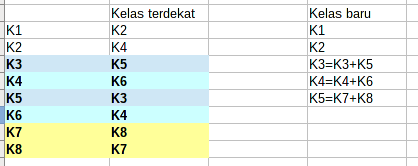
\includegraphics[width=7.5cm]{tex/cmerge7.png}
\caption{Penggabungan Kelas}
\label{fig:neighborhood}
\end{figure}

\subsection{Klasifikasi Ulang \emph{Pixel} ke Kelas Baru}

\emph{Pixel} diklasifikasikan ulang ke kelas-kelas baru yang diperoleh dengan metode \emph{nearest neighbor}. Perhitungan jarak yang digunakan adalah \emph{sum of squared difference} untuk tiap komponen warna.

\begin{equation}
ssd(p,k) = \sqrt{\frac{\sum_{r,g,b} (\mu(k) - p)^2}{3}}
\end{equation}

\section{Deteksi dan Pengukuran Prosentase Cacat Kulit Jeruk}

%\subsection{Pembentukan \emph{Mask}}

\emph{Pixel} yang diklasifikasikan dalam kelas dengan rata-rata intensitas tertinggi merupakan daerah normal pada kulit jeruk. Untuk menandainya dilakukan operasi \emph{thresholding} pada matriks kelas \emph{pixel} dengan nilai kelas tertinggi sebagai nilai \emph{threshold}.

Contoh pembentukan mask $M$ dari matriks kelas $K$ dengan kelas 5 sebagai kelas dengan rata-rata intensitas tertinggi.

\begin{equation*}
M  = \begin{bmatrix}
1 & 1 & 1 & 1 & 1 \\
1 & 5 & 5 & 5 & 1 \\
1 & 5 & 1 & 5 & 1 \\
1 & 4 & 5 & 3 & 1 \\
1 & 1 & 1 & 1 & 1
\end{bmatrix} \qquad 
K  = \begin{bmatrix}
0 & 0 & 0 & 0 & 0 \\
0 & 1 & 1 & 1 & 0 \\
0 & 1 & 0 & 1 & 0 \\
0 & 0 & 1 & 0 & 0 \\
0 & 0 & 0 & 0 & 0
\end{bmatrix}
\end{equation*}

%\subsection{Operasi \emph{Hole Filling}}

Penandaan daerah cacat memerlukan penentuan seluruh daerah jeruk yang bisa diproses dengan metode ini. Daerah tepi dengan kelas yang intensitasnya lebih rendah tidak dapat diproses karena perbedaan perbandingan nilai intensitas antara daerah normal dan daerah cacat. Bagian tepi tersebut tidak dimasukkan ke dalam perhitungan.

Untuk mendapatkan seluruh daerah yang tercakup pemrosesan maka dilakukan operasi morfologis \emph{hole filling} pada \emph{mask} daerah normal.

\begin{align}
	p_{cacat} = & \frac{L_{cacat}}{L_{normal} + L_{cacat}} \\
	L_{normal} \approx & Luas(H) \\
	L_{cacat} \approx & Luas(H' - H)
\end{align}

%$H'$ adalah \emph{convex hull} semua \emph{pixel} $H$ yang masuk dalam kelas dengan intensitas tertinggi.
$H$ adalah kumpulan \emph{pixel} dengan kelas yang paling tinggi intensitasnya, $H'$ adalah hasil pengisian lubang. Cacat dideteksi dari selisih antara $H$ dan $H'$.

\section{Akurasi Deteksi}

Akurasi deteksi cacat akan diukur dari parameter presisi, \emph{recall} dan akurasi statistik jumlah \emph{pixel} daerah cacat dan daerah normal. Hal-hal ini terkait dengan keberhasilan sistem dalam mengambil informasi yang dibutuhkan pengguna. Pada penelitian ini informasi yang dicari adalah \emph{pixel} dari daerah cacat.

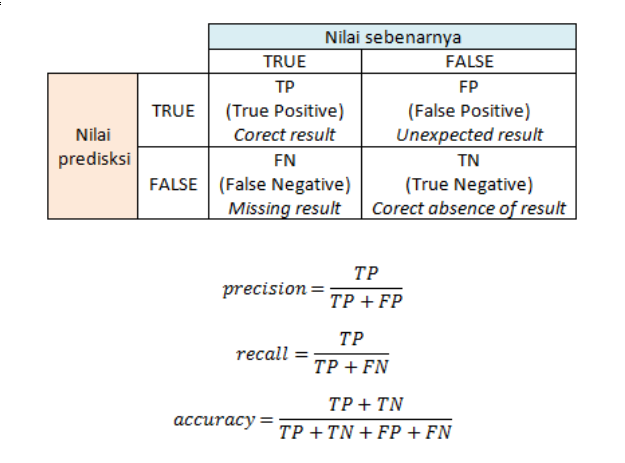
\includegraphics[width=8cm]{tex/conf.png}


\begin{enumerate}
\item \emph{True positive rate}: jumlah \emph{pixel} daerah cacat yang berhasil dideteksi oleh algoritma
\item \emph{False positive rate}: jumlah \emph{pixel} daerah normal yang ditandai sebagai cacat.
\item \emph{True negative rate}: jumlah \emph{pixel} daerah normal yang tidak ditandai sebagai cacat, 
\item \emph{False negative rate}: jumlah \emph{pixel} daerah cacat yang tidak terdeteksi oleh algoritma.
\end{enumerate}

Selain itu ditambahkan lagi ukuran prosentase deteksi yang dirumuskan sebagai perbandingan antara luas daerah yang dapat diproses dari tiap citra jeruk dengan luas keseluruhan objek jeruk yang tampak. Prosentase deteksi ini tidak akan mencapai 100\% karena bagian tepi objek jeruk menerima lebih sedikit cahaya intensitas warnanya lebih rendah dan tidak terdeteksi sebagai kelas tertinggi (daerah normal).

\begin{equation}
	deteksi = \frac{Luas(H')}{\sum_{kelas>1}^n Luas(M_{kelas})}
\end{equation}

$H'$ merupakan hasil pengisian lubang yang menunjukkan bagian yang dapat diproses, $M_{kelas}$ merupakan mask hasil klasifikasi akhir jeruk.

\end{document}
